% Milan Marcinčo - 120845 | Metódy inžinierskej práce

\documentclass[10pt,twoside,slovak,a4paper]{article}

\usepackage[slovak]{babel}
%\usepackage[T1]{fontenc}
\usepackage[IL2]{fontenc}
\usepackage[utf8]{inputenc}
\usepackage{graphicx}
\usepackage{url}
\usepackage{hyperref}
\usepackage{float}
\usepackage{cite}
%\usepackage{times}

\pagestyle{plain}

\title{Cloud gaming\thanks{Semestrálny projekt v predmete Metódy inžinierskej práce, ak. rok 2022/23, vedenie: Ing. Zuzana Špitálová}}

\author{Milan Marcinčo\\[2pt]
	{\small Slovenská technická univerzita v Bratislave}\\
	{\small Fakulta informatiky a informačných technológií}\\
	{\small \texttt{xmarcinco@stuba.sk}}
	}

\date{\small 13. december 2022}



\begin{document}

\maketitle

\begin{abstract}
Vývoj v oblasti technológií a informatiky ako takej napreduje ohromnou rýchlosťou už dlhé roky, a to bez akýchkoľvek náznakov približovania sa k stropu. Ruka v ruke s ním rastie aj náročnosť počítačových hier a požiadavky na parametre hardvéru. Staršie generácie procesorov a grafických kariet už nedokážu poskytovať dostatočný výpočtový výkon pre nové herné tituly a vyžadujú si častú výmenu za nový, moderný kus. Jedným z možných riešení tohto problému je hranie v cloude (cloud gaming), čím sa zaoberá aj tento článok. Jedná sa o konceptovo veľmi jednoduchý, ale realizačne veľmi zložitý prístup. S aktuálne dostupnými technológiami a ich rozšírením má hranie v cloude mnoho zraniteľných miest a prekážok na ceste k dokonalosti.
\end{abstract}



\section{Úvod}

\subsection{Čo je to cloud gaming?}

\paragraph{} Cloud gaming alebo všeobecnejšie cloud computing je veľmi atraktívne, moderné riešenie pre hráčov dnešnej doby, vo forme predplatnej služby. Jedným z hlavných faktorov pri výbere nových komponentov hernej zostavy je okrem výkonu aj cena, ktorá vďaka globálnemu nedostatku čipov v nedávnej minulosti niekoľkokrát prekonala svoje predošlé maximá. Oblasť, v ktorej služba hrania v cloude vyniká, je práve pomer ceny, výkonu a aktuálnosti hardvéru, na ktorom herné tituly bežia. Tú si na svoju zodpovednosť berie poskytovateľ služby, čo je pre koncového používateľa veľkou výhodou.



\subsection{Ako to funguje?}

\paragraph{} Hlavná myšlienka, na ktorej celé hranie v cloude stojí, je presun výkonovo náročných výpočtových operácií z používateľovho osobného počítača do cloudu. Každému hráčovi sú v čase hrania priradené hardvérové prostriedky, vrátane procesorových jadier, pamäte RAM, jadier grafickej karty a úložného priestoru, zvyčajne typu SSD. Tieto prostriedky sú využívané na všetky výpočty potrebné k behu hry a enkódovanie výstupného obrazu. Takto zakódované video je potom po internetovej sieti v reálnom čase streamované do počítača koncového používateľa, kde je následne zobrazené. Rovnakým spôsobom je prenášaný aj vstup z klávesnice, myši a iných vstupných periférií do cloudu, kde je spracovávaný a kde ovplyvňuje priebeh hry a jej výstupný obraz.\cite{6882299}

\paragraph{} V praxi to znamená, že počítač na strane používateľa je vyťažovaný len dekódovaním výstupného obrazu hry a spracovávaním a odosielaním vstupov, na čo je vo výsledku potrebný len zlomok výpočtového výkonu. To dovoľuje používateľovi použiť pri hraní v cloude takmer akékoľvek zariadenie, aj so staršími a pomalšími komponentami.

\begin{figure}[H]
	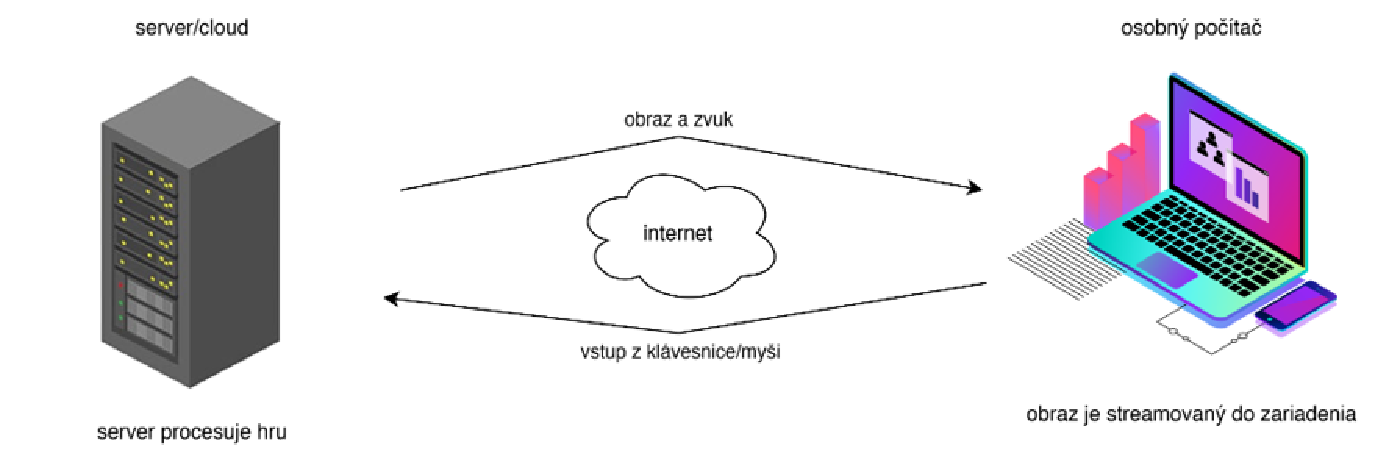
\includegraphics[width=1.0\textwidth]{diagram.pdf}
	\caption{Znázornenie konceptu hrania v cloude\cite{6882299}}
	\label{fig:cloud-gaming-concept}
\end{figure}



\section {Analýza}

\paragraph{} Keďže je cloud gaming len jednou z viacerých alternatív ako dosiahnúť akýsi herný zážitok, je dôležité vedieť si vybrať ten správny spôsob. Preto si v tejto sekcii bližšie rozoberieme a rozanalyzujeme silné a slabé stránky hrania v cloude, a porovnáme si niektoré z dostupných platforiem medzi sebou.

\subsection{Výhody oproti konvenčným herným zostavám}

\paragraph{} Hranie hier ako ho poznáme dnes je tu s nami už dlhé roky. Nové spôsoby a prístupy, ako napríklad hranie v cloude, musia byť vlasnosťami a funkcionalitou dostatočne atraktívne na to, aby dokázali zaujať a pretiahnuť na svoju stranu dostatočne veľkú masu hráčov. To sa dá dosiahnuť len vtedy, ak daný koncept dokáže ponúknuť značné výhody, ako napríklad: \cite{10.1007/978-981-10-6620-7_71}

\begin{itemize}

\item Odpadá nutnosť vlastniť drahý, výkonný počítač a pravidelne ho modernizovať, čo značne zníži nie len počiatočné, ale celkové náklady počas niekoľkých rokov.

\item Ukladanie progresu hry umožňuje pokračovať v hraní na rôznych zariadeniach z akéhokoľvek miesta, kde je stabilné internetové pripojenie.

\item Veľkosť úložného priestoru nehrá rolu, a tak nie je limitom pre množstvo hier, z ktorých si môže používateľ vybrať. Týmto je zároveň značne zvýšená efektivita, keďže nepotrebuje každý používateľ osobitnú kópiu celej hry, ale je zdieľaná celým datacentrom.

\item O funkčnosť a správny beh hardvéru sa stará poskytovateľ. Odpadajú tak akékoľvek starosti so servisom a zárukou hardvéru pre koncového užívateľa.

\end{itemize}



\subsection{Nevýhody a slabé stránky cloudu}

\paragraph{} Keďže sa celá podstata hrania v cloude a cloudu všeobecne točí okolo internetového pripojenia, môžeme očakávať, že práve to bude v tomto prípade tým najslabším článkom. \cite{10.1007/978-981-10-6620-7_71}

\begin{itemize}

\item V prípade neoptimálnej stability internetového pripojenia je zážitok z hier, najmä akčného multiplayer typu, viditeľne zníženy. Keďže sa všetky výpočty odohrávajú mimo počítača koncového užívateľa, každá akcia má nejakú odozvu, ktorá je v prípade týchto typov hier značné citeľná.

\item Stabilné internetové pripojenie je stále v mnohých častiach sveta nedostupné, alebo je veľmi nákladné. V tomto prípade hranie v cloude už nie je múdrou alternatívou, a častokrát ani možné.

\item Závislosť na prevádzkovateľovi služby je taktiež možnou nevýhodou. Akýkoľvek výpadok alebo útok na poskytovateľa znamená pre koncového používateľa neschopnosť službu využívať.

\end{itemize}



\subsection{Dostupné platformy a ich porovnanie}

\paragraph{} Existuje viacero dostupných platforiem, ktorých cieľom je poskytovať cloud gaming služby po celom svete. Avšak keďže je hranie v cloude pomerné nový koncept, môžeme predpokladať, že najkvalitnejšie platformy budu práve tie, ktoré sú financované a vyvíjané niektorou z popredných, veľkých spoločností. Preto sa pozrieme na päť najznámejších poskytovateľov, a to GeForce Now, Google Stadia, Xbox Cloud, Playstation Now a Amazon Luna. Porovnáme si kvalitu streamovania, veľkosť knižníc dostupných hier a unikátne vlastnosti každej z týchto platforiem, ktoré používatelia môžu považovať za veľké plus. \cite{geforce-now}\cite{stadia}\cite{xbox-cloud}\cite{playstation-now}\cite{amazon-luna}

\begin{figure}[H]
	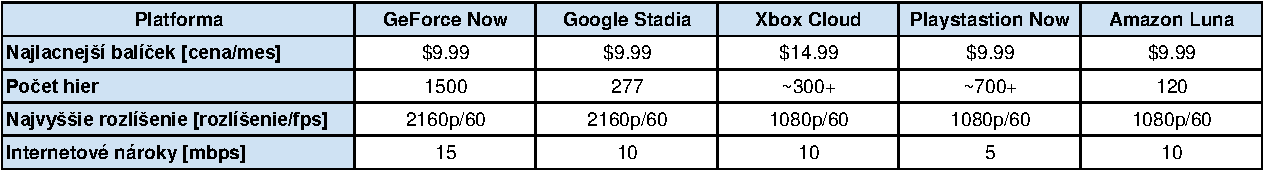
\includegraphics[width=1.0\textwidth]{cloud-gaming-tabulka-crop.pdf}
	\caption{Porovnanie dostupných platforiem \cite{geforce-now}\cite{stadia}\cite{xbox-cloud}\cite{playstation-now}\cite{amazon-luna}}
	\label{fig:comparison-table}
\end{figure}

\subsubsection{Kvalita streamovania}

\paragraph{} Rozlíšenie 1920x1080 pixelov, zvané aj ako "Full HD" rozlíšenie, sa stalo už akýmsi bežným štandardom v hraní na konvenčných herných zostavách. A to najmä vďaka dostatočnému množstvu detailov, ktoré dokážu na tomto rozlíšení vyniknúť, a nízkych výkonnostných nárokoch na grafickú kartu počítača. Vďaka svojej dlhšej existencií máme záruku, že bude podporované takmer všetkými platformami. Internetové nároky sa hýbu zväčša v rozmedzí 10 až 15 megabitov za sekundu.

\paragraph{} O stupeň vyššie, rozlíšenie "Quad HD", teda 2560x1400 pixelov, je pri hraní hier takzvanou zlatou strednou cestou. Ponúka výborný pomer detailov, zatiaľ čo výkonnostné nároky sú stále rozumne vysoké. Z našich piatich porovnávaných platforiem ho ponúkajú len dve, a to GeForce Now od spoločnosti Nvidia a Google Stadia.

\paragraph{} Prémiové, 4K rozlíšenie, 3840x2160 pixelov, ponúkajú taktiež iba platformy s najschopnejšou infraštruktúrou. Z nášho výberu to sú Geforce Now od Nvidie a Stadia od Googlu. Toto rozlíšenie ponúka najvyšší level zobrazenia detailov, avšak s razantne zvýšenými výkonnostnými a internetovými nárokmi. Najnovšie hry pri tomto rozlíšení dokážu zvládnuť len tie najmodernejšie a najpokročilejšie grafické karty. Pre plynulý obraz je na prenos výstupu z cloudu do počítača používateľa potrebné veľmi stabilné internetové pripojenie o rýchlosti najmenej 35 až 40 megabitov za sekundu.

\subsubsection{Knižnica dostupných hier a jedinečné vlastnosti jednotlivých platforiem}

\paragraph{} Medzi jednotlivými porovnávanými platformami sú v počte hier priepastné rozdiely. Dôležitý je aj spôsob, akým prichádzame k vlastníctvu kópií hier, ktorý sa taktiež medzi rôznymi poskytovateľmi líši. Práve tieto dva faktory najviac ovplyvnia výber platformy u nádejného zákazníka.

\paragraph{} Dôvodom, prečo si platforma GeForce Now môže pripísať titul služby s najväčšou hernou knižnicou je, že ponúkajú možnosť spárovať si službu s používateľovým vlastným Steam účtom. Pre koncového zákazníka to znamená, že môže svoju zbierku hier zdieľať medzi klasickým počítačom u seba doma, a zároveň aj so svojím účtom u poskytovateľa služby hrania v cloude.

\paragraph{} Opačný prístup zvolila služba Stadia od Googlu. Výber je síce značne zúžený, ale za to ponúkajú určitý čas na vyskúšanie akejkoľvek hry. Na základe toho sa môže zákazník následne rozhodnúť, či si hru zakúpi. V prípade že sa tak stane, bude táto hra prístupná len v službe Stadia.

\paragraph{} Zlatú strednú cestu ponúka Xbox Cloud, kde je v cene mierne vyššieho mesačného poplatku zahrnutá celá dostupná knižnica. Používateľ si tak môže slobodne vybrať akúkoľvek hru, bez akejkoľvek ďalšej platby. Veľkým plusom je však aj možnosť hrania týchto hier mimo cloudu.



\subsection{Výzvy a prekážky}

\paragraph{} Existuje mnoho prekážok, ktoré musia platformy ponúkajúce služby hrania v cloude prekonať. Jednou z mnoha výziev je problém s odozvou, čo v praxi znamená, že všetky akcie hráča majú určité oneskorenie predtým, než sa zobrazia na obrazovke. To môže byť ešte viac problematické ak sa jedná o hry akčného typu, kde je akákoľvek latencia ľahko citeľná, čo môže rýchlo viesť k úplne neakceptovateľnej skúsenosti. \cite{4591393} \cite{10.1145/1016540.1016557}

\subsubsection{Možné riešenia}

\paragraph{Servery na hrane - edge servers} Jedným z viacerých spôsobov ako znížiť latenciu pri hraní v cloude je použitie takzvaných serverov na hrane. Pod pojmom server na hrane sa myslí skutočný, fyzický server umiestnený k hráčovi oveľa bližšie v porovnaní s hlavným herným serverom. Tieto servery sú využívané na spracovanie časti hráčovho vstupu a video výstupu vo fyzicky menšej vzdialenosti, čo napomáha znížiť veľkost a trvanie prenosu dát do hlavného servera, a tým pádom taktiež znížiť odozvu. \cite{8289317}

\paragraph{Video kodek s nízkou latenciou} Kodek, teda spôsob akým je video enkódované a dekódované, môže mať taktiež obrovský vplyv na jeho výslednú veľkosť, a teda aj prenosovú rýchlosť a latenciu. Je preto veľmi dôležité, aby bol kodek nie len správne zvolený, ale aj optimalizovaný pre dané použitie. Pri prenose veľkého množstva dát, čo je v prípade hrania v cloude samozrejmosť, môže aj zanedbateľný rozdiel vo veľkej mierke spôsobiť komplikácie s efektívnosťou.

\paragraph{} Vo všeobecnosti, snaha znížiť latenciu je veľmi komplexný problém vyžadujúci kombináciu nie len technických riešení, ale aj optimizácie na strane používateľa a internetovej infraštruktúry ako celku.



\section{Zhodnotenie a záver}

\subsection{Cieľová skupina používateľov}

\paragraph{} Hranie v cloude je pre každého, kto rád trávi svoj voľný čas hraním videohier, ale nemá prístup k potrebnému hardvéru, ktorý by zvládol aj tie najnovšie a najzaujímavejšie hry. Vďaka hraniu v cloude môže používateľ jednoducho streamovať akékoľvek hry na požiadanie, a to aj bez výkonného herného počítača alebo konzoly. Taktiež, hranie v cloude môže byť skvelou voľbou pre niekoho, kto chce hrať na množstve rôznych zariadení, vrátane mobilov, tabletov a moderných televízorov.

\subsection{Cloud gaming ako budúcnosť herného priemyslu?}

\paragraph{} Je veľmi náročné predvídať budúcnosť herného priemyslu, keďže sa neustále evolvuje a mení. Avšak, technológia hrania v cloude už teraz má potrebný potenciál značne ovplyvniť priemysel a smer, akým napreduje. Trávenie času hraním hier je tak prístupnejšie a oveľa pohodlnejšie. Až časom sa uvidí, akú bude mať táto technológia adopciu, a ako bude integrovaná do hernej scény ako celku. \cite{7182690}



\section{Vyjadrenie k témam z prednášok}

\paragraph{Načo budem inžinierom (bakalárom)?} Inžinieri hrajú v dnešnom svete kľúčovú rolu. Oni su tí, ktorí vymýšľajú, navrhujú a realizujú systémy a technológie, bez ktorých by sme si dnešný svet nevedeli predstaviť. O to viac je to pravda v oblasti informatiky, kde sú práve inžinieri zodpovední za dizajn a vývoj hardvérových a softvérových systémov potrebých pre spracovávanie, uchovávanie a prenos informácií. V dnešnom svete, kde nie len naše životy, ale aj obrovská časť celosvetovej ekonomiky záleží na schopnosti pristupovať a využívať informácie rýchlo a efektívne, je táto funkcia veľmi kritická. Ďalšou náplňou práce inžinierov je aj stále vylepšovať a zefektívnovať existujúce systémy a vyvíjať nové technológie tak, aby nám pomohli vyriešiť tie najväčšie výzvy, ktorým ako ľudstvo čelíme. Skvelým príkladom oblasti, v ktorej je práca inžinierov potrebná je práve aj cloud gaming. Cloudové technológie sú už teraz na veľmi dobrej úrovni, avšak ešte stále je priestor na zlepšenie.

\paragraph{Vedecké publikovanie v informatike. Plagiátorstvo a ako sa mu vyhnúť.} Plagiátorstvo sa v oblasti informatiky, tak ako v ktorejkoľvek inej oblasti, vo všeobecnosti považuje za závažné porušenie pravidiel, aj morálky. Aj keď je pravda, že vývoj je v informatike vo veľkej miere založený na abstrakcii a stavaní na už objavených princípoch, stále však platí, že je potrebné citovať a korektne sa odkazovať na prácu iných ľudí, ak na ňu nadväzujeme alebo z nej využívamé akékoľvek poznatky a pozorovania. Privlastňovať si niečo, čomu iný človek venoval dlhé hodiny práce môže značne ovplyvniť reputáciu, a je veľmi ťažké znovu si vydobiť dôveru.

\paragraph{} V prípade, že počas zbierania ideí a zhromažďovania informácií a faktov posúvame odkazovanie sa na použitú literatúru bokom, môže ľahko dôjsť aj k nechcenému plagiátorstvu. Čím rozsiahlejšia práca je, tým ľahšie je stratiť sa v kope informácií, či nevedomky vydávať cudzí nápad za svoj. Ľudská myseľ nie je dokonalá, a preto je dôležité viesť si presný a štruktúrovaný zoznam použitej literatúry a inšpirácií už pred začiatkom písania.

\paragraph{História informatiky} Informatika ako veda má síce bohatú, ale zase nie až tak dlhú históriu. Od prvých počítačov, veľkých ako niekoľko miestností, neubehli storočia, ale len niekoľko pár desiatok rokov. V dobe, keď sa takéto počítače využívali najmä pre vedecké a vojenské účely, nikomu ani len nenapadlo, že jedného dňa bude mať každý jeden z nás takýto kus technológie vo vrecku. Nie len že sú počítače dnes menšie, tenšie, ľahšie a elegantnejšie, ale hlavne sú nepredstaviteľne rýchlejšie. Nie je vôbec divu, že sa postupom rokov mobily a osobné počítače rozšírili medzi obrovské masy ľudí. Takémuto rapídnemu vývoju vďačíme aj za to, že viedol k rozšíreniu internetu a napredovaniu aj v mnohých, úplne iných oblastiach, bez ktorých by sme si dnešný svet nevedeli predstaviť. Nech už ide o akékoľvek aspekty moderného života, od komunikácie a zábavy, po vzdelávanie a zdravotníctvo, môžeme byť neskutočne hrdí na to, o aký veľký krok sme sa vďaka našej vynaliezavosti posunuli.



\bibliography{literatura}
\bibliographystyle{plain}
\end{document}
